%
% Apunte de Sistemas Operativos
% Copyright (C) 2014 Esteban De La Fuente Rubio (esteban[at]delaf.cl)
%
% Permission is granted to copy, distribute and/or modify this document
% under the terms of the GNU Free Documentation License, Version 1.3
% or any later version published by the Free Software Foundation;
% with no Invariant Sections, no Front-Cover Texts, and no Back-Cover Texts.
% A copy of the license is included in the section entitled "GNU
% Free Documentation License".
%
% Link: http://www.gnu.org/copyleft/fdl.html
%

% CAPÍTULO PROCESOS
\chapter{Procesos}
\label{procesos}
La definición más simple para describir un proceso corresponde a un
\textbf{programa en ejecución}. Es importante notar que el proceso no es solo el
código, sino que es el código más los datos que conforman al proceso, su pila,
registros del procesador, descriptores de E/S, etc, en general cualquier dato
que permita administrar el proceso. Veremos que esto último es conocido como
contexto del proceso.

Adicionalmente se debe considerar que un proceso para ser ejecutado, deberá ser
planificado por el sistema operativo, de esta forma podrá hacer uso de la CPU
por un período determinado de tiempo. Lo anterior ocurre ya que el proceso
está siendo ejecutado con otros procesos y debe compartir los recursos,
incluyendo la CPU.

\section{Distribución de la memoria}
Todo proceso que se ejecuta dentro del sistema operativo, utilizando una MMU,
verá direcciones virtuales. En estas direcciones virtuales se ordena la memoria
del proceso a partir de las direcciones más bajas como se muestra en la figura
\ref{fig:memoria_proceso}.

\begin{itemize}

	\item \textbf{Código del programa}: instrucciones en código de máquina a
	ejecutar por el proceso.

	\item \textbf{Datos}: área para variables globales, inicializadas o no
	inicializadas.

	\item \textbf{\textit{Stack}}: área para datos de funciones.

	\item \textbf{\textit{Heap}}: espacio utilizado para la asignación
	dinámica de memoria, por ejemplo mediante \texttt{malloc}.

\end{itemize}

Existen implementaciones donde el \textit{stack} y el \textit{heap} están
invertidos y el \textit{stack} crece hacia las direcciones  bajas de la memoria
virtual.

\begin{figure}[htbp]
\centering
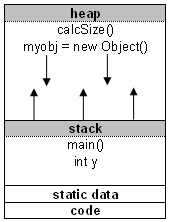
\includegraphics[scale=1.00]{img/C04_procesos/HeapAndStack}
\caption{Distribución de la memoria}
\label{fig:memoria_proceso}
\end{figure}

Las direcciones virtuales que no se encuentran asignadas al proceso, o sea
donde no hay un mapeo de dichas direcciones virtuales a direcciones físicas no
se pueden utilizar. Por lo cual si un proceso trata de acceder arbitrariamente
a una zona ilegal de memoria, donde no hay asignación o en algunos sistemas al
área del código se producirá una \textbf{\textit{segmentation fault}}. A
continuación se muestra un ejemplo de código que podría generar este error:

\lstinputlisting{codigo/C04_procesos/segmentation_fault.c}

En caso de un \textit{segmentation fault} el sistema generará una interrupción
llamada dirección ilegal, el sistema operativo determina la causa y envía una
señal al proceso indicando el error ocurrido. Si esta señal no es capturada por
el proceso hijo, entonces el proceso padre, muchas veces la \textit{shell},
recibirá la señal y mostrará el mensaje ``Segmentation fault'', el proceso hijo
terminará y el padre (\textit{shel}) continuará su ejecución.

En direcciones virtuales superiores, se encuentra la memoria del sistema, la
cual es solo accesible en modo sistema. Cuando ocurre una interrupción, el
núcleo atrapará la interrupción y el sistema operativo ejecutará, según el
vector de interrupciones, las instrucciones que atienden dicha interrupción.
Esta parte de la memoria, corresponde al núcleo del sistema operativo la cual
esta siempre residente en memoria y es ``compartida'' entre los procesos. Un
proceso normal no puede ver el área de código del sistema operativo, solo se
accede cuando hay un cambio a modo sistema. Ningún código que no pertenezca al
sistema deberá ejecutarse en dicha área de memoria, ya que de hacerlo implicaría
ejecución en modo sistema.

\section{Contexto}
El sistema operativo para gestionar el sistema requiere de diferentes datos, los
cuales se organizan en \textit{tablas}, ejemplo de estas tablas son:

\begin{enumerate}[i.]

	\item \textbf{Tabla de memoria}: asignación de memoria principal (RAM),
	asignación de memoria secundaria (almacenamiento), atributos de
	protección o de compartición y datos para la gestión de memoria virtual.

	\item \textbf{Tabla de E/S}: disponibilidad de recursos, estado de las
	operaciones de E/S y porción de memoria principal usada como
	origen/destino (\textit{buffers de E/S}).

	\item \textbf{Tabla de archivos}: existencia de archivos, posición en
	memoria secundaria, estado actual y otros atributos.

	\item \textbf{Tabla de procesos}: contexto del proceso.

\end{enumerate}

De esta última tabla, la de procesos, nos preocuparemos a continuación.

El \textbf{contexto}, imagen o descriptor del proceso corresponde a todos los
datos que el sistema operativo requiere para realizar la administración del
proceso. Este contendrá diversos datos referentes al estado de ejecución
del proceso.

El contexto será una estructura de datos que representará al proceso,
conteniendo datos del mismo, como por ejemplo cuantos milisegundos de CPU ha
usado el proceso en modo sistema o en modo usuario. El comando \texttt{time}
entrega el tiempo en modo usuario (\textit{user}) y modo sistema (\textit{sys}).
Las interrupciones que ocurren son contabilizadas en el tiempo del proceso que
ocurren, las cuales no necesariamente son del proceso que se esta ejecutando.
Un ejemplo de ejecución del comando time para un proceso de compilación es el
siguiente:

\begin{verbatim}
$ time gcc -Wall codigo.c -o programa
real    0m0.082s
user    0m0.052s
sys     0m0.020s
\end{verbatim}

\subsection{Atributos del proceso}
A continuación se listan algunos de los elementos que pueden ser encontrados
dentro del contexto de un proceso.

\subsubsection{Identificación del proceso}
\begin{itemize}

	\item Identificador del proceso.

	\item Identificador del proceso padre.

	\item Identificador del usuario.

\end{itemize}

El identificador del proceso o \textbf{PID} corresponde a la identificación
pública de un proceso. El Sistema operativo administra una tabla que permite
asociar el PID hacia la dirección donde se encuentra el contexto del proceso.
Los procesos entre sí se conocen únicamente por su PID.

\subsubsection{Información del estado del procesador}
\begin{itemize}

	\item Registros visibles para el usuario: aquellos que se pueden
	referenciar mediante el lenguaje de máquina.

	\item Registros de control y estado: aquellos utilizados por el
	procesador para ejecutar el código, ej: \textit{program counter}.

	\item Punteros de pila: apunta a la cima de la pila.

\end{itemize}

\subsubsection{Información de control del proceso}
\begin{itemize}

	\item Información de planificación y estado: estado, prioridad, sucesos
	u otros.

	\item Estructuración de datos: enlaces entre procesos, ejemplo:
	colas por estar bloqueados.

	\item Comunicación entre procesos: señales, mensajes, tuberías.

	\item Privilegios: memoria, tipo de instrucciones, servicios o
	utilidades del sistema.

	\item Gestión de memoria: punteros hacia las direcciones de memoria
	asignadas.

	\item Propiedad sobre recursos: recursos controlados por el proceso,
	ejemplo: archivos abiertos.

\end{itemize}

\subsection{Cambios de contexto}
El \textbf{cambio de contexto} de un proceso ocurre cuando el proceso que se
está ejecutando sale de la CPU y entra uno nuevo. Lo anterior ya que cada
proceso necesita su propio contexto para la ejecución del mismo, por lo cual el
que está almacenado debe ser limpiado y cargado el nuevo.

Si un proceso está ejecutando operaciones de entrada y salida, y los datos
asociados a estas operaciones no están en \textit{buffers} el proceso no
puede continuar, por lo cual debe bloquearse, entregar el control al sistema
operativo y el \textit{scheduler} tomará el control escogiendo otro proceso que
si pueda continuar, en ese momento ocurre un cambio de contexto entre los
procesos (el que sale por estar bloqueado y el que entra por estar listo). Lo
mismo ocurre cuando se acaba el tiempo mediante la interrupción del cronómetro
regresivo, ya que al no poder seguir usando la CPU el proceso debe salir y
entrar uno diferente (asumiendo que hay más procesos listos).

Suponga el siguiente escenario: tiene un proceso en ejecución en la CPU al cual
todavía le queda tiempo del asignado, sin embargo el sistema operativo debe
atender una interrupción que llegó por alguna razón. Al ser una interrupción el
proceso en ejecución será interrumpido y se pasará a ejecutar la parte de código
en el área de sistema, todo esto en el tiempo de ejecución del proceso que está
en la CPU. Luego de atender la interrupción se continuará con el proceso por el
tiempo que le queda disponible.

Es importante mencionar que una interrupción podría originar un cambio de
contexto, pero no necesariamente. Por ejemplo en el caso del cronómetro
regresivo se generará una interrupción que implicará cambio de contexto, pero
un aviso del disco duro enviando una interrupción informando que los datos
están ubicados en el \textit{buffer} no generará cambio de contexto. De todas
formas siempre esto tiene que ver con las políticas y mecanismos ya que un
sistema operativo podría generar un cambio de contexto ante una interrupción que
otro no lo genera.

Los cambios de contexto son caros ya que se debe limpiar la memoria donde
se almacena el mismo, y esto al acceder al hardware, es lento. Luego de limpiar
se debe restaurar el contexto de interés (escribiendo en la memoria).

Al realizar un cambio de contexto se debe:
\begin{itemize}

	\item Resguardar los registros del proceso que sale.

	\item Contabilizar el uso de CPU.

	\item Cambiar de espacio de direcciones virtuales. Usualmente implica
	invalidar caché de nivel 1, lo cual es lo más costoso, esto es así en
	los procesos pesados y deben su nombre justamente a esto.

	\item Resguardar los registros del proceso que entra.

\end{itemize}

\section{Estados}
Durante la ejecución de un proceso este puede encontrarse en diferentes estados,
se debe comprender que el proceso al iniciar su ejecución no siempre se estará
\textit{ejecutando}, ya que deberá compartir el tiempo de CPU con otros procesos
en el sistema, e inclusive con el mismo sistema operativo, el cual también es un
proceso en ejecución. Adicionalmente pueden ocurrir otras situaciones que lleven
al proceso de un estado a otro.

Los diferentes estados pueden ser vistos en la figura
\ref{fig:procesos_estados}. A continuación se describirán estos y los motivos
que pueden llevar a pasar de uno a otro durante la ejecución del proceso.

\begin{figure}[htbp]
	\centering
	\selectlanguage{english}
	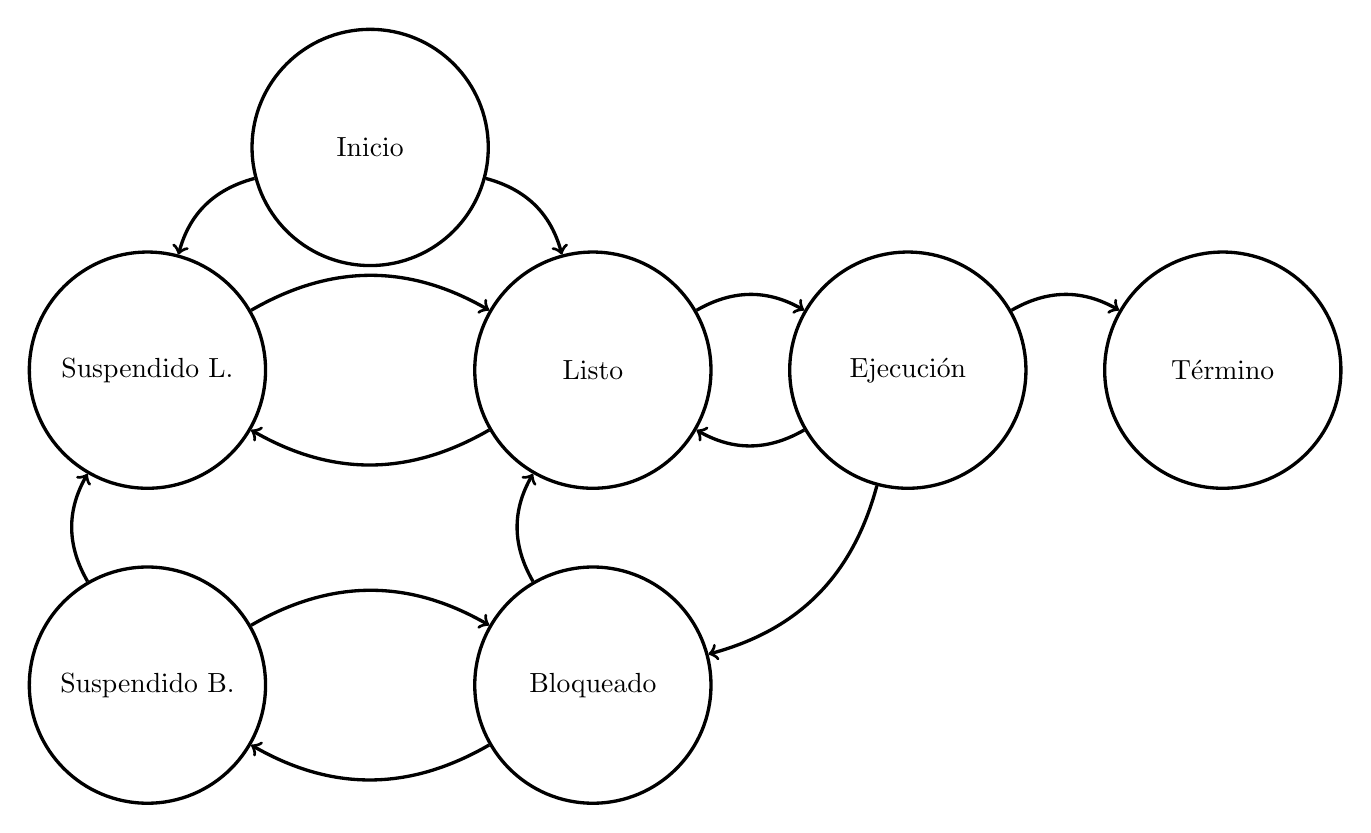
\begin{tikzpicture}
		% formatos
		\tikzstyle{every node} = [auto, node distance=4cm, semithick]
		\tikzstyle{node} = [draw, circle, minimum size=3cm, very thick]
		\tikzstyle{arrow} = [->, very thick]
		% nodos
		\node [node] (inicio) {Inicio};
		\node [node] (listo) [below right of =inicio] {Listo};
		\node [node] (ejecucion) [right of =listo] {Ejecución};
		\node [node] (termino) [right of =ejecucion] {Término};
		\node [node] (bloqueado) [below of =listo] {Bloqueado};
		\node [node] (s_listo) [below left of =inicio] {Suspendido L.};
		\node [node] (s_bloqueado)[below of =s_listo] {Suspendido B.};
		% relaciones
		\draw [arrow] (inicio) to [bend left] node {} (listo);
		\draw [arrow] (inicio) to [bend right] node {} (s_listo);
		\draw [arrow] (s_listo) to [bend left] node {} (listo);
		\draw [arrow] (listo) to [bend left] node {} (s_listo);
		\draw [arrow] (listo) to [bend left] node {} (ejecucion);
		\draw [arrow] (ejecucion) to [bend left] node {} (listo);
		\draw [arrow] (ejecucion) to [bend left] node {} (termino);
		\draw [arrow] (ejecucion) to [bend left] node {} (bloqueado);
		\draw [arrow] (bloqueado) to [bend left] node {} (listo);
		\draw [arrow] (bloqueado) to [bend left] node {} (s_bloqueado);
		\draw [arrow] (s_bloqueado) to [bend left] node {} (bloqueado);
		\draw [arrow] (s_bloqueado) to [bend left] node {} (s_listo);
	\end{tikzpicture}
	\selectlanguage{spanish}
	\caption{Estados de un proceso}
	\label{fig:procesos_estados}
\end{figure}

Cuando se lanza un programa a ejecución, el proceso no necesariamente comienza a
ejecutarse inmediatamente, sino que pasará por un estado de \textbf{inicio},
donde se deberán realizar distintas operaciones que tienen que ver con la
preparación del entorno para la ejecución del proceso.

Una vez que se ha creado el entorno del proceso, y existe memoria para que este
pueda comenzar, pasa a estado \textbf{listo} donde espera a ser planificado para
entrar a la CPU y ejecutar su código.

Al momento de ser elegido el proceso para su ingreso a la CPU pasa a estado de
\textbf{ejecución}. Donde se encontrará, en una primera instancia, hasta que el
tiempo asignado por el sistema operativo expire. Una vez el tiempo expire el
proceso volverá a estado listo, donde volverá a esperar para ser planificado.

Si durante la ejecución del proceso este requiere algún recurso que no está
disponible, el proceso pasará a estado \textbf{bloqueado} hasta que el sistema
operativo le indique que el recurso que está solicitando le fue asignado. Como
se vió anteriormente, esto podría ser por ejemplo una lectura de datos desde el
disco. Una vez se asigna el recurso el proceso pasará a estado listo nuevamente
con el recurso ya disponible para ser utilizado la próxima vez que entre a la
CPU.

Una vez el proceso haya cumplido con la ejecución de su programa, o haya
ocurrido algún evento que lleve al proceso a su estado final, se encontrará en
estado de \textbf{término} o estado \textit{zombie}, donde el proceso ya terminó
su ejecución pero aun no se han liberado sus recursos. Esto es utilizado, por
ejemplo, por un proceso padre que requiere datos una vez el proceso haya
terminado, por lo cual será la llamada a \texttt{wait} del proceso padre la que
liberará finalmente los recursos del proceso \textit{zombie}.

Las razones de término de un proceso no solo se deben porque terminó con la
ejecución de su código, a continuación se mencionan otras causas:
\begin{itemize}
	\item Límite de ejecución excedido.
	\item Límite de espera excedido.
	\item No hay memoria disponible.
	\item Violación de segmento (o límites).
	\item Error de protección.
	\item Error aritmético.
	\item Error E/S.
	\item Instrucción inválida.
	\item Instrucción privilegiada.
	\item Mal uso de datos.
	\item Intervención del SO.
	\item Terminación del padre.
	\item Solicitud del padre.
\end{itemize}

Con los estados descritos hasta ahora un sistema podría funcionar, sin embargo
¿qué sucedería si en un determinado momento el sistema tiene muchos procesos
bloqueados y otros nuevos esperando entrar a estado listo? Con el esquema
descrito hasta ahora, si la RAM estuviese completamente ocupada nuevos procesos
no podrían ser recibidos. Considerando esto es que aparecen dos estados
adicionales, \textbf{suspendido listo} y \textbf{suspendido bloqueado}, los
cuales se encargarán de mover a un almacenamiento secundario los procesos que
por alguna razón no puedan ser llevados a estado listo. Si un proceso se
encuentra bloqueado será llevado a bloqueado suspendido para que espere sin
consumir RAM por el recurso que está solicitando, en cambio si un proceso es
nuevo y no hay memoria RAM podrá ser iniciado en un estado suspendido listo,
donde ya tendrá su contexto y solo faltará memoria principal para poder ser
candidato a planificación.

El sacar un proceso de la CPU y colocar otro en esta implicará diversos pasos,
los cuales se mencionan a continuación:
\begin{enumerate}

	\item Guardar el contexto del proceso que sale.

	\item Actualizar el bloque de control del proceso que sale.

	\item Mover el bloque de control a la cola adecuada (según estado en que
	quedó el proceso que sale).

	\item Seleccionar otro proceso para ejecución (planificación).

	\item Actualizar el bloque de control del proceso seleccionado (cambiar
	a ejecución).

	\item Actualizar las estructuras de datos de gestión de memoria.

	\item Restaurar el contexto del proceso, incluyendo los
	registros del procesador a aquel estado que existía cuando el proceso
	seleccionado dejó el procesador la vez anterior.

\end{enumerate}

Nos preocuparemos especialmente de los algoritmos de planificación más adelante.

\section{Clasificación de procesos}
Los procesos pueden clasificarse en dos grupos básicos, como \textbf{procesos
pesados} y como \textbf{procesos livianos}. Cada uno tendrá sus características,
ventajas y desventajas. En el cuadro \ref{tab:procesos_clasificacion} se pueden
apreciar sus similitudes y diferencias.

\begin{table}[hbt]
	\centering
	\begin{tabular}{|c|c|c|}
		\hline
						& Pesado			& Liviano \\
		\hline
			Jerga			& procesos Unix			& threads \\
			Implementación		& fork				& hebras \\
			Espacio de direcciones	& propio  			& compartido \\
			Archivos		& compartido			& compartido \\
			Procesador		& propio (1)			& propio (varios) \\
			Requisitos de hardware	& MMU, interrupciones y timers	& interrupciones y timers \\
			Protección		& si				& no \\
			Comunicaciones		& mensajes, sockets, pipes	& memoria compartida (punteros) \\
			Costo cambio contexto	& alto				& bajo \\
			Ejeplos	de S.O.		& Unix e IBM VM370		& AmigaOS, MacOS y Win 3.11 \\
		\hline
	\end{tabular}
	\caption{Comparativa entre procesos pesados y livianos}
	\label{tab:procesos_clasificacion}
\end{table}

Notar que la comparación se hace pensando en la ejecución de varios procesos
pesados en paralelo en un sistema operativo, o bien la ejecución de un único
proceso liviano con muchas hebras ejecutándose de forma paralela.

En sistemas operativos \textit{like Unix} tradicionalmente se han utilizado
procesos pesados. Si bien POSIX entrega una implementación de hebras, esto es
más ``moderno'', en los tiempos iniciales solo habían procesos pesados.

Sistemas operativos \textit{de juguete} por lo general utilizan procesos
livianos, ya que el sistema operativo en sí corre sobre un proceso pesado de
Unix.

Sistemas operativos como Unix modernos, Linux o WIndows 2000 y NT hacia adelante
pueden proveer tanto procesos pesados como livianos.

\subsection{Procesos \textit{preemptive} y \textit{non-preemptive}}
Adicionalmente a la clasificación anterior el sistema operativo puede ofrecer,
una de estás opciones, procesos de tipo \textit{preemptive} y
\textit{non-preemptive}.

\subsubsection{Procesos \textit{preemptive}}
Los procesos \textbf{\textit{preemptive}} son aquellos donde el núcleo puede
quitar la CPU a un proceso en cualquier momento, esto mediante interrupciones.

Ejemplos de este tipo de sistema son sistemas \textit{like Unix} y Windows NT y
posteriores.

\subsubsection{Procesos \textit{non-preemptive}}
En los procesos \textbf{\textit{non-preemptive}} es el proceso quien decide
invocar al núcleo y devolver el control al sistema operativo. En estos casos
debe haber una cooperación entre las aplicaciones y el sistema operativo para
ofrecer paralelismo.

Ejemplo de este tipo de sistema son Windows 3.11 y MacOS antes de la versión
6.X. Los sistemas operativos mencionados no estaban diseñados para la ejecución
simultánea de varias aplicaciones, siendo las aplicaciones quienes debían
implementar mecanismos de sincronización.

La principal ventaja de esta forma de ejecución de procesos es que son fáciles
de programar. Como desventaja se tiene que sin un proceso se queda en un
\textit{loop} infinito la única solución es reiniciar la máquina.

\section{Paralelismo}
Un sistema con multiprocesador será capaz de ejecutar procesos en paralelo, en
este caso se están considerando varios \textit{chips}. Otra alternativa
corresponde a un sistema multinúcleo, donde existe un solo chip de procesador el
cual posee varias CPU (núcleos).

En general, lo que hará el sistema operativo será emular el multiprocesamiento,
ya que si bien se puede contar con un procesador con 2 o 4 núcleos, o más,
siempre se querrá tener más procesos en ejecución que la cantidad de núcleos que
la máquina pueda proveer. En estos sistemas se entregarán tajadas de tiempo,
donde cada proceso dispondrá de un tiempo finito y determinado para ejecutar su
código, de no alcanzar deberá intentarlo más tarde nuevamente.

Si bien este paralelismo solo se podría lograr al disponer de un sistema con
múltiples procesadores se debe recordar que los tiempos son tan pequeños que al
ejecutarse todos los procesos da la sensación que ocurren en paralelo.

El concepto de concurrencia está relacionado con la ejecución en
\textit{paralelo} de los procesos. La \textbf{concurrencia} aparecerá al
ejecutarse procesos en paralelo, donde dos o más procesos querrán acceder al
mismo tiempo a un determinado recurso. Originalmente la única programación con
múltiples procesos era la del sistema operativo, ya que los lenguajes no
entregaban soporte para concurrencia. Pero hoy en día, como los lenguajes si
ofrecen concurrencia como parte del lenguaje o biblioteca es importante conocer
lo que esta implica.

Independientemente de si estamos trabajando en un sistema multiprocesador,
multinúcleo o con emulación del paralelismo existirán problemas relacionados a
este \textit{paralelismo}. Los cuales tendrán directa relación con la forma en
que se ejecutan los procesos. Se discutirán a continuación los problemas que
pueden ocurrir en un ambiente con múltiples procesos en ejecución, los cuales
corresponden a \textit{data races}, \textit{deadlocks} y \textit{starvation}. En
el capítulo \ref{sincronizacion} se verán métodos de sincronización que
permitirán controlar estas situaciones.

\subsection{\textit{Data races}}
Los \textbf{\textit{data races}} o condición de carrera (\textit{race
condition}) ocurre en un proceso cuando se obtiene un estado inconsistente del
sistema, o bien cuando los datos que se obtienen se encuentran en un estado
inconsistente. La idea de carrera se puede considerar como dos o más procesos
que compiten para producir cierto estado final del sistema.

Considere el siguiente código:
\begin{lstlisting}
/* parte global (comun a todos los hilos) */
int contador = 0;
/* codigo principal de cada hilo en ejecucion */
void aumentar ()
{
  int aux = contador; /* instruccion 1 */
  contador = aux + 1; /* instruccion 2 */
}
\end{lstlisting}

Suponga que la función \texttt{aumentar()} se está ejecutando en forma
paralela en dos hilos (hebras o \textit{threads}), ¿qué problema se podría
presentar?. Se debe considerar que las operaciones de la función no son
atómicas, o sea pueden ser divididas, por lo tanto el sistema operativo puede
interrumpir al proceso y detener su ejecución en cualquier línea de ejecución
del código\footnote{Se ha forzado el código a tener 2 líneas, sin embargo debe
considerar que aunque fuese una línea la operación será dividida en varias
operaciones al ser pasada a código de más bajo nivel}. Al existir la posibilidad
que el sistema operativo interrumpa la ejecución del código en cualquier parte
del código puede ocurrir la siguiente situación:

\begin{enumerate}[i.]

	\item Hilo 1 ejecuta la función \texttt{aumentar()}, guarda el
	valor del contador y es interrumpido. Entonces aux = 0.

	\item Hilo 2 ejecuta la función \texttt{aumentar()}, guarda el
	valor del contador y es interrumpido. Entonces aux = 0.

	\item Hilo 1 hace la suma y guarda el valor. Entonces contador = 1.

	\item Hilo 2 hace la suma y guarda el valor. Entonces contador = 1.

\end{enumerate}

Al final de la operación la variable contador tendrá el valor 1, ¿era el valor
esperado? ¿qué valor debiera tener la variable contador?.

El resultado esperado será inconsistente ya que se esperaba que después de la
ejecución de los dos hilos el contador tuviese valor 2. Sin embargo a causa de
la ejecución en paralelo y la no existencia de sincronización el valor
resultante es incorrecto. Este problema también es conocido como el problema de
\textbf{exclusión mutua}, ya que lo lógico que se esperaría es que mientras un
proceso modifica una sección crítica los otros no puedan hacerlo.

Este es, de los problema de concurrencia que se verán, el peor de todos ya que
son \textbf{difíciles de detectar} y son \textbf{no determinísticos}.
Adicionalmente entregan un resultado al usuario, uno incorrecto, con lo cual él
podría no darse cuenta si dicho resultado es o no el esperado.

\subsubsection{Agregar elementos a una pila o \textit{stack}}
\begin{lstlisting}
Pila p;
int indice = 0;
void agregar(Pila p, Objeto o)
{
  put(p, o, indice++);
}
\end{lstlisting}

\subsubsection{Sentarme en una silla}
\begin{lstlisting}
int sillas[10]; /* arreglo inicializado en 0 */
void sentarme ()
{
  int i;
  for(i=0; i<10; ++i) {
    if(sillas[i]==0) {
      sillas[i] = 1;
      me_siento(i);
      break;
    }
  }
}
\end{lstlisting}

Se debe evitar pensar que el orden de las instrucciones puede ayudar con los
problemas de \textit{data races}, ya que el compilador puede reordenar el código
secuencial dejándolo de una forma no deseada. La solución correcta es el uso de
alguna herramienta de sincronización, como semáforos, para garantizar la
exclusión mutua.

\subsection{\textit{Deadlock}}
Un \textbf{\textit{deadlock}} o interbloqueo corresponde a una situación donde
un proceso requiere cierto recurso que algún otro tiene asignado, pero el otro
proceso para continuar, y eventualmente liberar el recurso, requiere el que
tengo yo asignado. Esto se puede observar en la figura \ref{fig:interbloqueo}.

\begin{figure}[htbp]
	\centering
	\selectlanguage{english}
	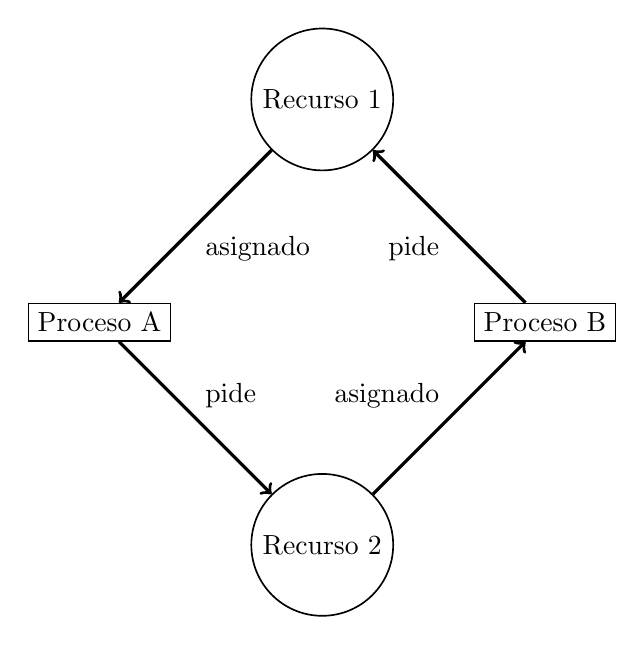
\begin{tikzpicture}
		% formatos
		\tikzstyle{every node}=[auto, node distance=4cm, semithick]
		\tikzstyle{arrow} = [->, very thick]
		% nodos
		\node [draw, circle] (R1) {Recurso 1};
		\node [draw] (PA) [below left of =R1] {Proceso A};
		\node [draw] (PB) [below right of =R1]	{Proceso B};
		\node [draw, circle] (R2) [below right of =PA] {Recurso 2};
		% relaciones
		\draw [arrow] (R1) to node {asignado} (PA);
		\draw [arrow] (PA) to node {pide} (R2);
		\draw [arrow] (R2) to node {asignado} (PB);
		\draw [arrow] (PB) to node {pide} (R1);
	\end{tikzpicture}
	\selectlanguage{spanish}
	\caption{Interbloqueo, espera circular entre proceso A y B}
	\label{fig:interbloqueo}
\end{figure}

Supongamos por un momento que tenemos una función que permite solicitar un
recurso y otra que permite liberar el recurso, más adelante veremos que esto es
posible hacerlo mediante herramientas como los semáforos. En este escenario se
propone la siguiente situación, donde Pa y Pb son dos procesos diferentes y que
se están ejecutando de forma paralela.

\begin{lstlisting}
Pa                       Pb
solicitar(S);            solicitar(Q);
solicitar(Q);            solicitar(S);
/* uso de Q y S en la seccion critica */
devolver(S);             devolver(Q);
devolver(Q);             devolver(S);
\end{lstlisting}

Si el proceso A se está ejecutando, solicita $S$, lo sacan de la CPU, entra el
proceso B y solicita $Q$. ¿Qué sucedera cuando entre nuevamente A y solicite
$Q$?. Ambos procesos estarán esperando que el otro libere el recurso que
necesitan.

Pensando en un ejemplo más concreto podría corresponder al problema:
\begin{lstlisting}
Servicio tenedor;
Servicio cuchillo;
function comer_asado()
{
  solicitar(tenedor);
  solicitar(cuchillo);
  comer();
  liberar(tenedor);
  liberar(cuchillo);
}
\end{lstlisting}

Para comer se requiere tanto el tenedor como el cuchillo y solo hay disponibles
uno de cada uno. ¿Qué podría ocurrir al haber dos personas tratando de comer?

Otro ejemplo puede ser el del puente colgante, donde:
\begin{itemize}

	\item Tráfico en una sola dirección.

	\item Cada sección del puente será un recurso.

	\item Si ocurre un \textit{deadlock}, uno de los usuarios deberá
	retroceder.

	\item Puede ser que varios usuarios deban retroceder.

	\item Puede haber inanición.

\end{itemize}

Para que ocurra interbloqueo se requieren las siguientes condiciones:
\begin{enumerate}

	\item Debe existir exclusión mutua.

	\item Los procesos deben mantener tomado el recurso y esperar por el
	siguiente.

	\item No debe existir apropiación por parte del sistema operativo
	(o sea que pueda quitarles el recurso).

	\item La espera debe ser circular.

\end{enumerate}

A continuación se mencionan posibles casos con los que el sistema operativo
podrá enfrentar un interbloqueo.

\subsubsection{Ignorar el problema}
\begin{itemize}

	\item Hacer como si el problema no existiera.

	\item Fundamento: bloqueos pueden ocurrir muy pocas veces, donde las
	políticas para solucionarlo pueden llevar a mecanismos complejos y que
	degraden el rendimiento del sistema.

	\item Unix utiliza este mecanismo.

\end{itemize}

\subsubsection{Detección y recuperación}
\begin{itemize}

	\item Permite que ocurran bloqueos.

	\item Cuando ocurren los detecta y lleva a cabo una acción para
	solucionarlo.

	\item Detección: ejecutar algoritmo cada X tiempo que verifique si
	existen interbloqueos.

	\item Recuperación:
	\begin{itemize}

		\item Apropiación: quitar el recurso y asignarlo al otro
		proceso.

		\item Rollback: volver el sistema hacia un punto donde no hay
		bloqueo.

		\item Eliminación del proceso: se eliminan procesos hasta romper
		el bloqueo.

	\end{itemize}

\end{itemize}

\subsubsection{Evitarlo dinámicamente}
\begin{itemize}

	\item Se hace una simulación de como quedaría el sistema si se asigna un
	recurso solicitado por un proceso.

	\item Se considera un estado seguro (todos satisfacen sus
	requerimientos) y uno inseguro (si uno o más procesos no podrán verse
	satisfechos).

	\item Si el estado en que queda la simulación es insegura, los recursos
	no serán asignados al proceso y deberá esperar.

	\item Algoritmo difícil de implementar, ya que procesos no conocen sus
	necesidades de recursos para un estado futuro.

\end{itemize}

\subsubsection{Evitar las cuatro condiciones}
Se busca que al menos una de las 4 condiciones necesarias para el bloqueo no se
cumpla.
\begin{itemize}

	\item Exclusión mutua: si los recursos no se asignaran de forma
	exclusiva a un proceso no habría problema de interbloqueos.

	\item Retención y espera: se debe evitar que procesos que ya tienen
	asignados recursos puedan solicitar nuevos sin liberar los que ya tienen
	(al menos temporalmente).

	\item No apropiación: quitar el recurso y asignarlo a otro (no siempre
	aplicable, ejemplo: impresora).

	\item Espera circular: los procesos deberán ordenarse para solicitar los
	recursos, no pudiendo hacerlo todos al mismo tiempo.

\end{itemize}

\subsection{\textit{Starvation}}
Una situación de \textbf{\textit{starvation}}, hambruna o inanición corresponde
a la situación donde por alguna razón un proceso no obtiene nunca el recurso
solicitado. Finalmente el proceso termina por tiempo de espera excedido, o sea,
muere de hambre. La existencia de hambruna permitirá tener un mayor
paralelismo.

Un ejemplo de esta situación:
\begin{itemize}
	\item Procesos A, B y C.
	\item Recurso R.
	\item Planificador asigna recurso R a A y B, pero nunca a C.
	\item C nunca adquiere el recurso para completar su objetivo y muere.
\end{itemize}

Para manejar el problema de inanición el sistema operativo puede asignar los
recursos mediante una cola FIFO o bien utilizar una prioridad para los procesos,
penalizando a quienes han adquirido el recurso y favoreciendo a quienes no. Esto
lo que busca es una asignación equitativa de los recursos, donde ninguno de los
procesos debe quedar sin ser atendido.

\section{Ejercicios y preguntas}
\begin{enumerate}

	\item ¿Qué compone a un proceso?.

	\item ¿Cuándo se ejecuta en CPU un proceso?.

	\item ¿Para qué se utiliza el espacio de memoria \textit{heap}?.

	\item ¿Para que se utiliza el espacio de memoria \textit{stack}?.

	\item ¿Qué es un \textit{segmentation fault}?.

	\item Describa a que corresponde el descriptor de un proceso.

	\item ¿Qué es el PID de un proceso?.

	\item ¿Qué información guarda el registro de CPU PC (\textit{program
	counter})?.

	\item Explique el proceso de cambio de contexto.

	\item ¿Cuáles son los estados de un proceso?, no es necesario que
	considere estados suspendidos.

	\item ¿Cuándo se pasa de estado listo a ejecución?.

	\item ¿Cuándo se pasa de estado ejecución a bloqueado?.

	\item ¿Cuándo se pasa de estado bloqueado a listo?.

	\item Indique 5 razones de término de un proceso.

	\item ¿Por qué es necesario el estado \textit{zombie} o terminado?.

	\item ¿Qué se debe restaurar cuando un proceso pasa de estado listo a
	ejecución?.

	\item Explique los proceso pesados y livianos, con sus ventajas y
	desventajas.

	\item Explique la diferencia entre procesos \textit{preemptive} y
	\textit{non-preemptive}.

	\item ¿Bajo que condición existe paralelismo en un sistema operativo?.

	\item Explique el problema de \textit{data races}.

	\item Explique el problema de \textit{deadlock}.

	\item Explique el problema de \textit{starvation}.

	\item Explique dos medidas que se puedan tomar frente a un interbloqueo.

	\item ¿Por qué el problema de \textit{data races} es considerado el mas
	complicado (malo) de los tres?.

\end{enumerate}

\section{Referencias}
\begin{itemize}

	\item Sistemas Operativos, Segunda Edición, Andrew Tanenbaum, Capítulo
	2.1.

	\item Sistemas Operativos, Quinta Edición, Abraham Silberschatz y Peter
	Baer Galvin, Capítulo 4.

	\item Sistemas Operativos, Segunda Edición, William Stallings, Capítulo
	3.

\end{itemize}
